\chapter{Intégration numérique}\index{Intégration numérique}
Ce chapitre traite le calcul numérique d’intégrales (§14.1) ainsi que la résolution
numérique d'équations différentielles ordinaires (§14.2) avec SymPy. Nous rappelons
des bases théoriques des méthodes d’intégration, puis nous détaillons les fonctions
disponibles et leur usage (§14.1.1). Le calcul symbolique d’intégrales avec SymPy a été traité précédemment (§2.3.8), et ne sera que mentionné rapidement ici comme une possibilité de calculer la
valeur numérique d’une intégrale. Cette approche « symbolique puis numérique »,
lorsqu’elle est possible, constitue une des forces de SymPy et est à privilégier car le
nombre de calculs effectués, et donc d’erreurs d’arrondi, est en général moindre
que pour les méthodes d’intégration numérique. Nous donnons une rapide introduction aux méthodes classiques de résolution d’équations différentielles, puis le traitement d’un exemple (§14.2.1) débutera l’inventaire des fonctions disponibles en SymPy (§14.2.2).

On s’intéresse au calcul numérique d’intégrales de fonctions réelles ; pour une
fonction $f : I \longrightarrow R$, où $I$ est un intervalle de $\mathbb{R}$, on veut calculer :
\[
\int_{I} f\left(x\right).
\]

Par exemple, calculons
\[
 \int_{1}^{3} x^{2}e^{-x^{2}}\cos\left(x\right) dx.
\] 

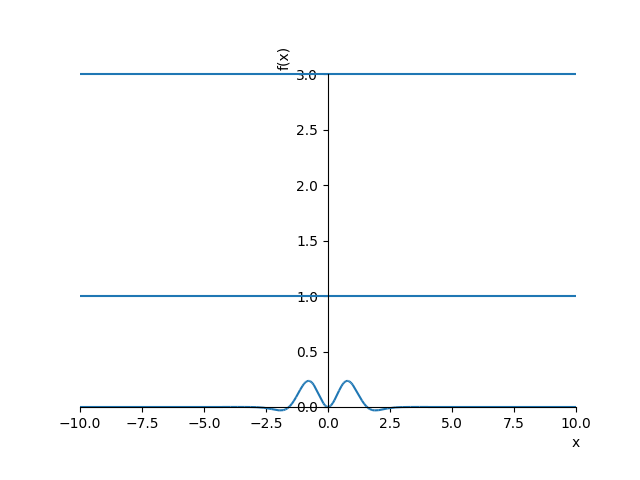
\includegraphics[scale=0.6]{../Pictures/Figure_1.png} 
\begin{python}
from sympy.abc import x
from sympy import integrate
from sympy.plotting import plot
f = x**2*exp(-x**2)*cos(x)
N(integrate(f, (x, 1, 3))
0.0306905101632536
plot(f, (1, 3, fill='axis'))
\end{python}

La fonction integrate calcule l’intégrale symbolique de l’expression, il faut
demander explicitement une valeur numérique pour l’obtenir.
\\
Il est aussi, en principe, possible de calculer des intégrales sur un intervalle
dont les bornes sont infinies :
\begin{python}
from sympy.abc import x
from sympy import sin, oo
N(integrate(sin(x**2)/(x**2), (x, 1, oo))
0.285736646322853
plot(sin(x**2)/(x**2), x, 1, 10, fill='axis')
\end{python}

\subsection{Equation and Text}\index{Examples!Equation and Text}

\begin{example}
Let $G=\{x\in\mathbb{R}^2:|x|<3\}$ and denoted by: $x^0=(1,1)$; consider the function:
\begin{equation}
f(x)=\left\{\begin{aligned} & \mathrm{e}^{|x|} & & \text{si $|x-x^0|\leq 1/2$}\\
& 0 & & \text{si $|x-x^0|> 1/2$}\end{aligned}\right.
\end{equation}
The function $f$ has bounded support, we can take $A=\{x\in\mathbb{R}^2:|x-x^0|\leq 1/2+\epsilon\}$ for all $\epsilon\in\intoo{0}{5/2-\sqrt{2}}$.
\end{example}

